\chapter{Verschmutzung des Drehtellers}
\section{Anforderungen und Ziele}
In Regelmäßigen Abständen soll der Verschmutzungsgrad des Drehtellers von einer Kamera erfasst und ausgewertet werden. Dabei sollen alle anstehenden und laufenden Befüll-Routinen angehalten werden, bis eine entsprechende Säuberung durchgeführt wurde.

\section{Vorgehen}
Um mögliche Komplikationen zu minimieren führen wir die Schmutzerkennung direkt vor jeder Befüll-Routine durch. Dabei ist die Kamera auf die Endposition der Gläser ausgerichtet.

Grund dafür ist die erhöhte Wahrscheinlichkeit, dass man den Inhalt des Glases beim Entnehmen verschüttet, weshalb die größte Verschmutzungsdichte eben dort zu erwarten ist. 

Vorteil davon ist, dass wir ebenfalls im Blick haben, ob das fertig befüllte Glas der vorherigen Routine beim Start einer neuen eventuell noch nicht entnommen wurde. Dies hätte zur Folge, dass ein volles Glas mit der Fotokammer kollidiert, was natürlich unerwünscht ist.

\subsection{Positionierung der Kamera}
\begin{wrapfigure}{rt}{0.6\linewidth}
	\centering
	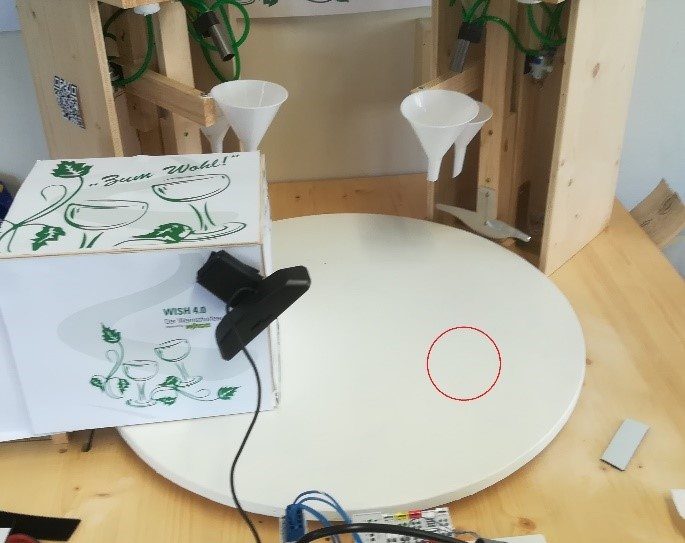
\includegraphics[width=\linewidth]{content/pictures/position_der_Kamera_zu_Schmutz}
	\caption{Positionierung der Kamera zur Schmutzerkennung}
	\label{fig:position_der_kamera_zu_schmutz}
\end{wrapfigure}
Um den Endbereich der Routine (Abbildung \ref{fig:position_der_kamera_zu_schmutz}, rechts), optimal zu Erfassen bringen wir die Kamera an der Seite der Fotokammer an (Abbildung \ref{fig:position_der_kamera_zu_schmutz}, links). Durch diese Positionierung haben wir alle relevanten Bereiche im Blick, während wir den Hintergrund minimieren.

\subsection{Trainingsdaten sammeln}
Für diesen Anwendungsfall definieren wir 3 Klassen:
\begin{itemize}
	\item Sauber
	\item Verschmutzt
	\item Besetzt
\end{itemize}
Dazu haben wir zunächst für 6 unterschiedliche Gläser jeweils 50 Bilder auf-genommen, auf welchen die Gläser an der erwarteten Endposition stehen. Diese klassifizieren wir als „besetzt“ (Abbildung \ref{fig:trainingsdaten_schmutz}c).

Als zweites haben wir insgesamt 50 Fotos des sauberen Drehtellers in verschiedenen Positionen aufgenommen und diese als „sauber“ klassifiziert (Abbildung \ref{fig:trainingsdaten_schmutz}a).

Zum Schluss haben wir mit Weiß-, Rosé-, und Rotwein jeweils 50 Bilder auf-genommen, indem wir ein Glas befüllten und den Inhalt beim Aufnehmen verschütteten, wie es auch in Anwendung sehr wahrscheinlich passieren wird. Dieses Set klassifizieren wir als „verschmutzt“ (Abbildung \ref{fig:trainingsdaten_schmutz}b, Verschmutzung oben zu erkennen).

\begin{figure}[!h]
	\centering
	
\includegraphics[width=0.25\linewidth,angle=-90]{content/pictures/2}
	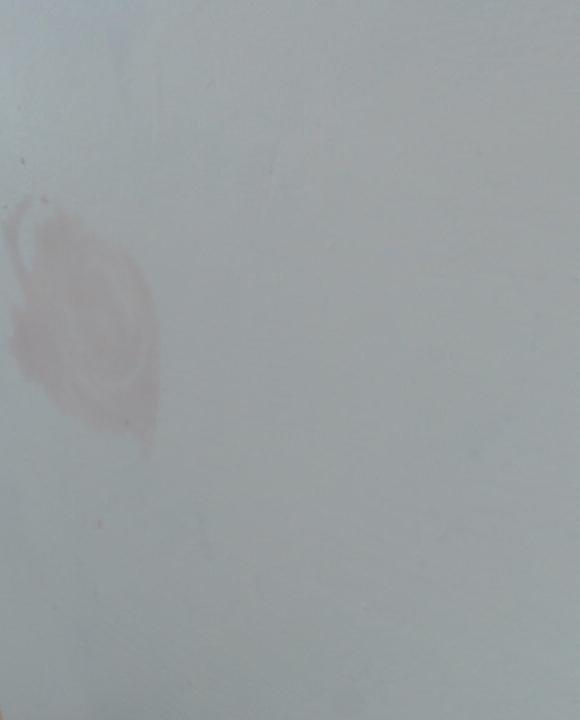
\includegraphics[width=0.25\linewidth,angle=-90]{content/pictures/1}
	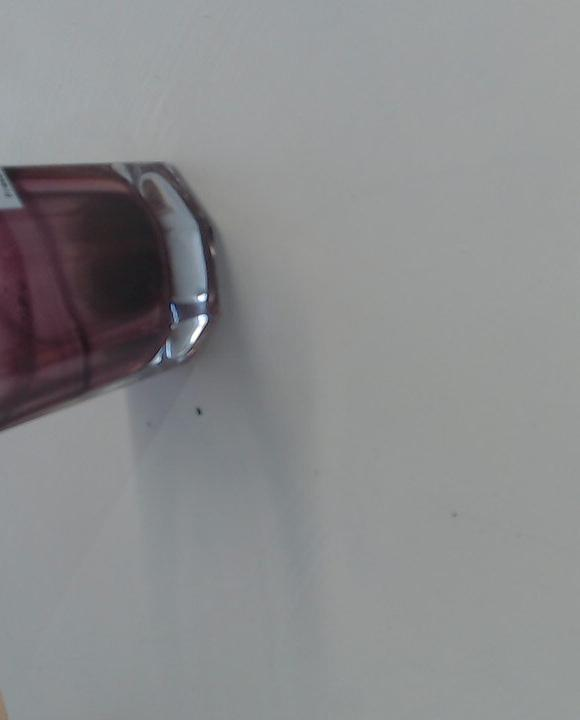
\includegraphics[width=0.25\linewidth,angle=-90]{content/pictures/0}
	\caption{Auszug aus den zugeschnittenen Trainingsdaten zur Verschmutzungserkennung (a) sauber, (b) verschmutzt und (c) besetzt}
	\label{fig:trainingsdaten_schmutz}
\end{figure}

\subsection{\ac{CNN}-Architektur}
Identisch zur Glaserkennung wird als Eingabe für das \ac{CNN} wir ein 3 Channel 128x128 Bild verwendet. 
Für die convolution Operationen setzen wir jedoch vier convolutional layer ein, um aus den schwerer zu unterscheidenden Bildern detailliertere Features herauszufiltern.
Dabei bestehen die ersten beiden layer aus 32, die anderen beiden layer aus 64 3*3 Filtern. 

Zur Erkennung sind gleich wie bei der Glaserkennung zwei FC-layer, die erste mit 128 Neuronen, die zweite mit 3 im Einsatz. Daraus ergibt sich die in Abbildung \ref{fig:table_structure} gezeigte Struktur des \ac{CNN}

\begin{figure}[!h]
	\centering
	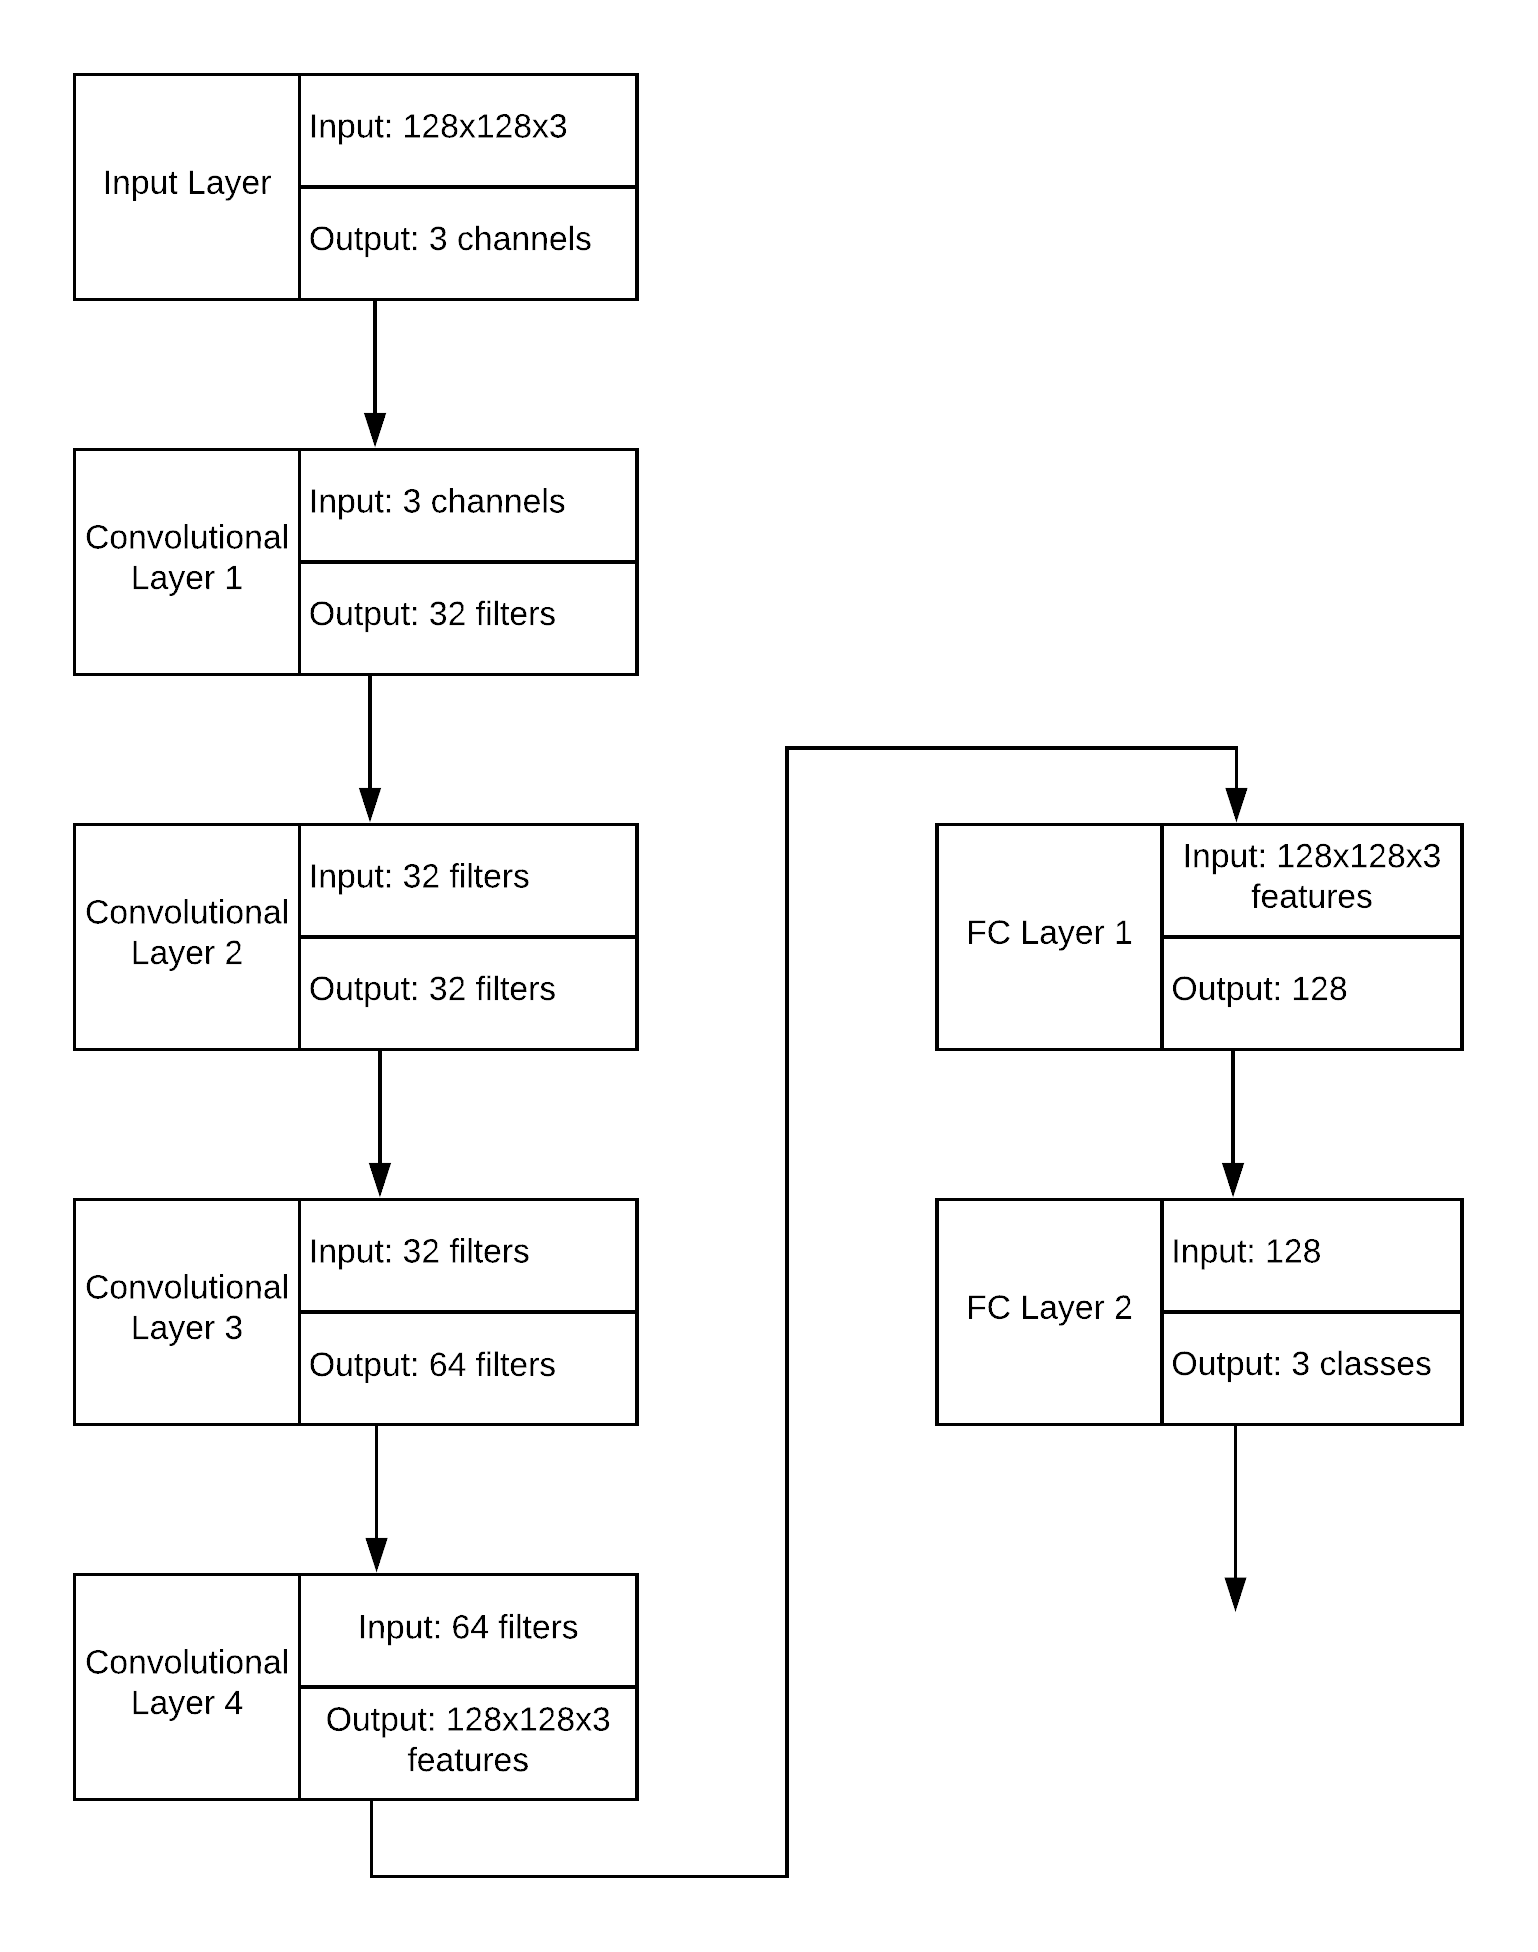
\includegraphics[width=0.7\linewidth]{content/pictures/table_structure}
	\caption{Struktur des \ac{CNN} zur Schmutzerkennung}
	\label{fig:table_structure}
\end{figure}
